\documentclass[a4paper,11pt]{article}
\input{/home/tof/Documents/Cozy/latex-include/preambule_lua.tex}
\newcommand{\showprof}{show them}  % comment this line if you don't want to see todo environment
\fancyhead[L]{Récursivité - exponentiation}
\newdate{madate}{10}{09}{2020}
\fancyhead[R]{Terminale - NSI} %\today
\fancyfoot[L]{~\\Christophe Viroulaud}
\fancyfoot[C]{\textbf{Page \thepage}}
\fancyfoot[R]{\includegraphics[width=2cm,align=t]{/home/tof/Documents/Cozy/latex-include/cc.png}}

\begin{document}
\begin{Form}
\section{Problématique}
$$a^n=\underbrace{a ×....× a}_{n fois}\qquad et\ a^0=1$$

Un calcul comme $3^4$ ne pose pas de problème mais $2701^{103056}$ peut prendre un certain à effectuer par le langage de programmation.
\begin{center}
\shadowbox{\parbox{13cm}{\centering Comment calculer la puissance d'un nombre de manière optimisée?}}
\end{center}
\section{Étude de la fonction native}
\subsection{Fonctions  Python "built-in"}
\begin{commentprof}
fournies par Python et/ou langages de haut-niveau.
\end{commentprof}
\begin{lstlisting}
def puissance_star(x:int,n:int)->int:
    return x**n

def puissance_builtin(x:int,n:int)->int:
    return pow(x,n)
\end{lstlisting}
\subsection{Tester un programme}
\subsubsection{Préconditions}
Nous nous limitons au cas positif.
\begin{commentprof}
évoquer la \emph{programmation défensive}
\end{commentprof}
\begin{activite}
Mettre en place un test qui lèvera une \emph{AssertionError} si l'exposant est négatif.
\end{activite}
\subsubsection{Mettre en place des tests}
Il existe plusieurs modules (\emph{doctest}) qui facilitent les phases de test. 
\begin{lstlisting}
import doctest

def puissance_star(x:int,n:int)->int:
    """
    >>> puissance_star(2,8)
    256
    >>> puissance_star(2,9)
    512
    """
    return x**n

doctest.testmod(verbose=True)
\end{lstlisting}
\subsection{Temps d'exécution}
Observons la durée d'exécution de nos fonctions, pour de grandes valeurs de paramètres.
\begin{lstlisting}
from time import time

debut=time()
puissance_star(2701,19406)
fin=time()
print("opérande **",fin-debut)
\end{lstlisting}
\section{Implémenter la fonction \emph{puissance}}
\subsection{S'appuyer sur la définition mathématique}
$$a^n=\underbrace{a ×....× a}_{n fois}\qquad et \qquad a^0=1$$
\begin{activite}
\begin{enumerate}
\item Implémenter la fonction \textbf{puissance\_perso(x: int, n: int)\;\rightarrow\;int} sans utiliser les fonctions buitin de Python.
\item Mettre en place un test de vérification de la fonction.
\item Mesurer le temps d'exécution de la fonction en l'appelant avec les paramètres (2701,19406).
\end{enumerate}
\end{activite}
\begin{commentprof}
\begin{lstlisting}
def puissance_perso(x:int,n:int)->int:
    """
    >>> puissance_perso(2,8)
    256
    >>> puissance_perso(2,9)
    512
    """
    res = 1
    for i in range(n):
        res*=x
    return res
\end{lstlisting}
\end{commentprof}
\subsection{Invariant de boucle}
Il permet de prouver la \emph{correction} d'un algorithme.\\
On appelle \emph{invariant d’une boucle} une propriété qui si elle est vraie avant l’exécution d’une itération le demeure après l’exécution de l’itération.\\
La propriété $res = x^i$ est un invariant de boucle. C'est en fait un raisonnement par récurrence comme en mathématiques.
\subsection{Temps d'exécution}
\begin{activite}
Que peut-on conclure à propos de l'implémentation de la fonction \emph{exponentielle} fournie par Python?
\end{activite}
\begin{commentprof}
durée ×20 par rapport aux fonctions builtin. Qu'en conclure?
\end{commentprof}
\section{Formulations récursives}
\subsection{Notation mathématique}
$$
puissance(x,n) = \left\{
    \begin{array}{ll}
        1 & \mbox{si } n=0 \\
        x.puissance(x,n-1) & \mbox{si } n>0
    \end{array}
\right.
$$
\subsection{Traduction en code}
\begin{lstlisting}
def puissance_recursif(x:int,n:int)->int:
    if n==0:
        return 1
    else:
        return x*puissance_recursif(x,n-1)
\end{lstlisting}
\begin{commentprof}
visualisation via pythontutor\\
tester sur petites valeurs\\
pour grandes valeurs: python limite la pile d'exécution à 1000 récursion\\
ne change rien pour la durée d'exécution pour l'instant.
\end{commentprof}
\subsection{Nouvelle formulation mathématique}
\begin{commentprof}
s'appuie sur les maths pour optimiser nos programmes//il y a une relation étroite maths/info (EDF recrute des matheux en Python)
\end{commentprof}
\begin{figure}[!h]
\centering
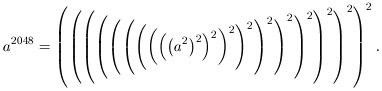
\includegraphics[width=7cm]{ressources/exponentiationrapide.png}
\captionof{figure}{Exponentiation rapide}
\label{exponentiation}
\end{figure}
$$
puissance(x,n) = \left\{
    \begin{array}{ll}
        1 & \mbox{si } n=0 \\
        puissance(x*x,n/2) & \mbox{si } n>0 \mbox{ et n pair}\\
        x.puissance(x*x,(n-1)/2) & \mbox{si } n>0 \mbox{ et n impair}\
    \end{array}
\right.
$$
\begin{lstlisting}
def puissance_recursif_rapide(x,n):
    if n==0:
        return 1
    elif n%2==0:
        return puissance_recursif_rapide(x*x,n//2)
    else:
        return x*puissance_recursif_rapide(x*x,n//2)
\end{lstlisting}
\begin{commentprof}
pourquoi n'obtient-on pas encore une durée similaire aux fonctions builtin? 
\begin{itemize}
\item Implémentation des fonctions builtin en C
\item itératif plus rapide car appels fonction coûtent; mais récursif donne souvent code plus clair/lisible
\item python pas optimisé pour récursif
\end{itemize}
code Python est opensource.\\on peut passer impératif <-> récursif
\end{commentprof}
\begin{lstlisting}
def puissance_iteratif_rapide(x,n):
    res=1
    while n>0:
        if n % 2 == 0:
            x = x*x
            n = n // 2
        else:
            res = res * x
            n = n - 1
    return res
\end{lstlisting}
\end{Form}
\end{document}